\documentclass[11pt,a4paper]{article}

% ---------- Pacotes ----------
% Compila tanto com pdfLaTeX quanto com XeLaTeX/LuaLaTeX
\usepackage{iftex}
\ifPDFTeX
  \usepackage[T1]{fontenc}
  \usepackage[utf8]{inputenc}
  \usepackage[brazil]{babel}
  \IfFileExists{tgpagella.sty}{\usepackage{tgpagella}}{\usepackage{mathpazo}}
\else
  \usepackage{fontspec}
  \usepackage{polyglossia}
  \setdefaultlanguage[variant=brazilian]{portuguese}
  \setmainfont{TeX Gyre Pagella}
\fi
\usepackage[a4paper,margin=2.5cm]{geometry}
\usepackage{microtype}
\usepackage{setspace}
\usepackage{xcolor}
\usepackage{titlesec}
\usepackage{fancyhdr}
\usepackage{amsmath}
\usepackage{graphicx}
\usepackage{float}
\usepackage{caption}
\usepackage{xurl}
\usepackage[hidelinks]{hyperref}
\urlstyle{same}

\definecolor{destaque}{HTML}{1F4E79}
\setstretch{1.25}
\setlength{\parindent}{1.25cm}
\setlength{\parskip}{0.35em}

% Legendas das figuras
\captionsetup{font={small,stretch=1.1},labelfont={bf,color=destaque},labelsep=period}

% Títulos das questões
\titleformat{\section}[hang]{\normalfont\large\bfseries\color{destaque}}{}{0pt}{}
\titlespacing*{\section}{0pt}{1.6em}{0.8em}

% Cabeçalho e rodapé
\pagestyle{fancy}
\fancyhf{}
\fancyhead[L]{\small\color{gray}CFD Ambientes Oceânicos -- Atividade 03}
\fancyhead[R]{\small\color{gray}Breno Santos Cabral}
\fancyfoot[C]{\small\thepage}
\renewcommand{\headrulewidth}{0.4pt}

\begin{document}

% ---------- Identificação ----------
\thispagestyle{empty}
\begin{center}
  {\Large\bfseries\color{destaque} CFD Ambientes Oceânicos}\\[0.3em]
  {\large Atividade 03}\\[0.8em]
  {\normalsize Breno Santos Cabral}\\[0.2em]
  {\small 30 de outubro de 2026}
\end{center}
\noindent\textcolor{destaque}{\rule{\textwidth}{0.8pt}}

% ---------- Metodologia ----------
\section{Metodologia}

O código \textsc{Fortran} fornecido foi reescrito na linguagem Python e pode ser acessado no link \url{https://github.com/BrenoSCabral/cfd_003}. O código avalia o desempenho de diferentes métodos numéricos na integração da equação

\begin{equation}
\frac{dU}{dt} = gU
\label{eq:cresc}
\end{equation}

\noindent cuja solução analítica é $U(t) = U_0\, e^{gt}$. Foram utilizados $g = 0{,}05$, $U_0 = 2$ e tempo total de integração de 300 unidades de tempo, com passos de tempo $\Delta t = 1$ e $\Delta t = 10$. Para cada método numérico, a discretização está destacada a seguir.

\textbf{Progressivo (Euler explícito)}
\begin{equation}
U^{n+1} = U^{n} + g U^{n} \Delta t
\end{equation}

\textbf{Runge-Kutta de 2ª ordem (RK2)}
\begin{equation}
\begin{aligned}
k_1 &= \Delta t \, g U^{n} \\
k_2 &= \Delta t \, g \left( U^{n} + \frac{k_1}{2} \right) \\
U^{n+1} &= U^{n} + k_2
\end{aligned}
\end{equation}

\textbf{Runge-Kutta de 4ª ordem (RK4)}
\begin{equation}
\begin{aligned}
k_1 &= \Delta t \, g U^{n} \\
k_2 &= \Delta t \, g \left( U^{n} + \frac{k_1}{2} \right) \\
k_3 &= \Delta t \, g \left( U^{n} + \frac{k_2}{2} \right) \\
k_4 &= \Delta t \, g \left( U^{n} + k_3 \right) \\
U^{n+1} &= U^{n} + \frac{1}{6}\left( k_1 + 2k_2 + 2k_3 + k_4 \right)
\end{aligned}
\end{equation}

\textbf{Leap-frog com filtro de Asselin}
\begin{equation}
\begin{aligned}
U^{n+1} &= \overline{U}^{\,n-1} + 2 g U^{n} \Delta t \\
\overline{U}^{\,n} &= U^{n} + \frac{\nu}{2}\left( \overline{U}^{\,n-1} - 2U^{n} + U^{n+1} \right)
\end{aligned}
\end{equation}

\noindent em que $\overline{U}$ representa o valor filtrado e $\nu = 0{,}2$ é o coeficiente do filtro. Por se tratar de um esquema de três níveis de tempo, o primeiro passo foi feito repetindo a condição inicial ($U^{1} = U^{0}$), como no código original.

\textbf{Matsuno}
\begin{equation}
\begin{aligned}
U^{*} &= U^{n} + g U^{n} \Delta t \\
U^{n+1} &= U^{n} + g U^{*} \Delta t
\end{aligned}
\end{equation}

\textbf{Heun}
\begin{equation}
\begin{aligned}
U^{*} &= U^{n} + g U^{n} \Delta t \\
U^{n+1} &= U^{n} + \frac{\Delta t}{2}\left( g U^{n} + g U^{*} \right)
\end{aligned}
\end{equation}

Como a Equação~\ref{eq:cresc} é linear, cada esquema de dois níveis pode ser escrito na forma $U^{n+1} = \lambda\,U^{n}$, em que $\lambda$ é o fator de amplificação. A solução exata, neste caso, corresponde a $\lambda = e^{g\Delta t}$. Diferentemente dos exemplos anteriormente tratados, espera-se que a solução cresça, devido à natureza do problema. A Tabela~\ref{tab:amplif} compara os fatores de amplificação de cada esquema com o valor exato. Para o leap-frog com filtro, o fator efetivo foi estimado numericamente pela razão $U^{n+1}/U^{n}$ ao final da integração.

\begin{table}[htbp]
\centering
\caption{Fator de amplificação por passo de tempo de cada esquema.}
\label{tab:amplif}
\begin{tabular}{lccc}
\hline
Esquema & $\lambda$ & $\Delta t = 1$ & $\Delta t = 10$ \\
\hline
Exato                  & $e^{g\Delta t}$ & 1,051271 & 1,648721 \\
Progressivo            & $1 + g\Delta t$ & 1,050000 & 1,500000 \\
RK2 / Heun             & $1 + g\Delta t + \frac{(g\Delta t)^2}{2}$ & 1,051250 & 1,625000 \\
RK4                    & $\sum_{k=0}^{4} \frac{(g\Delta t)^k}{k!}$ & 1,051271 & 1,648438 \\
Matsuno                & $1 + g\Delta t + (g\Delta t)^2$ & 1,052500 & 1,750000 \\
Leap-frog (com filtro) & -- & 1,051388 & 1,629563 \\
\hline
\end{tabular}
\end{table}

O erro relativo foi calculado como

\begin{equation}
\varepsilon^{n} = \frac{\left| U^{n} - U_a(t_n) \right|}{U_a(t_n)}
\end{equation}

\noindent em que $U_a$ é a solução analítica.

% ---------- Resultados e discussão ----------
\section{Resultados e discussão}

As soluções e os erros obtidos com $\Delta t = 1$ e $\Delta t = 10$ são apresentados nas Figuras~\ref{fig:dt1} e \ref{fig:dt10}, respectivamente. Os valores do erro relativo ao final da integração ($t = 300$) e a média ao longo de toda a integração estão apresentados na Tabela~\ref{tab:erros}.

\begin{figure}[H]
  \centering
  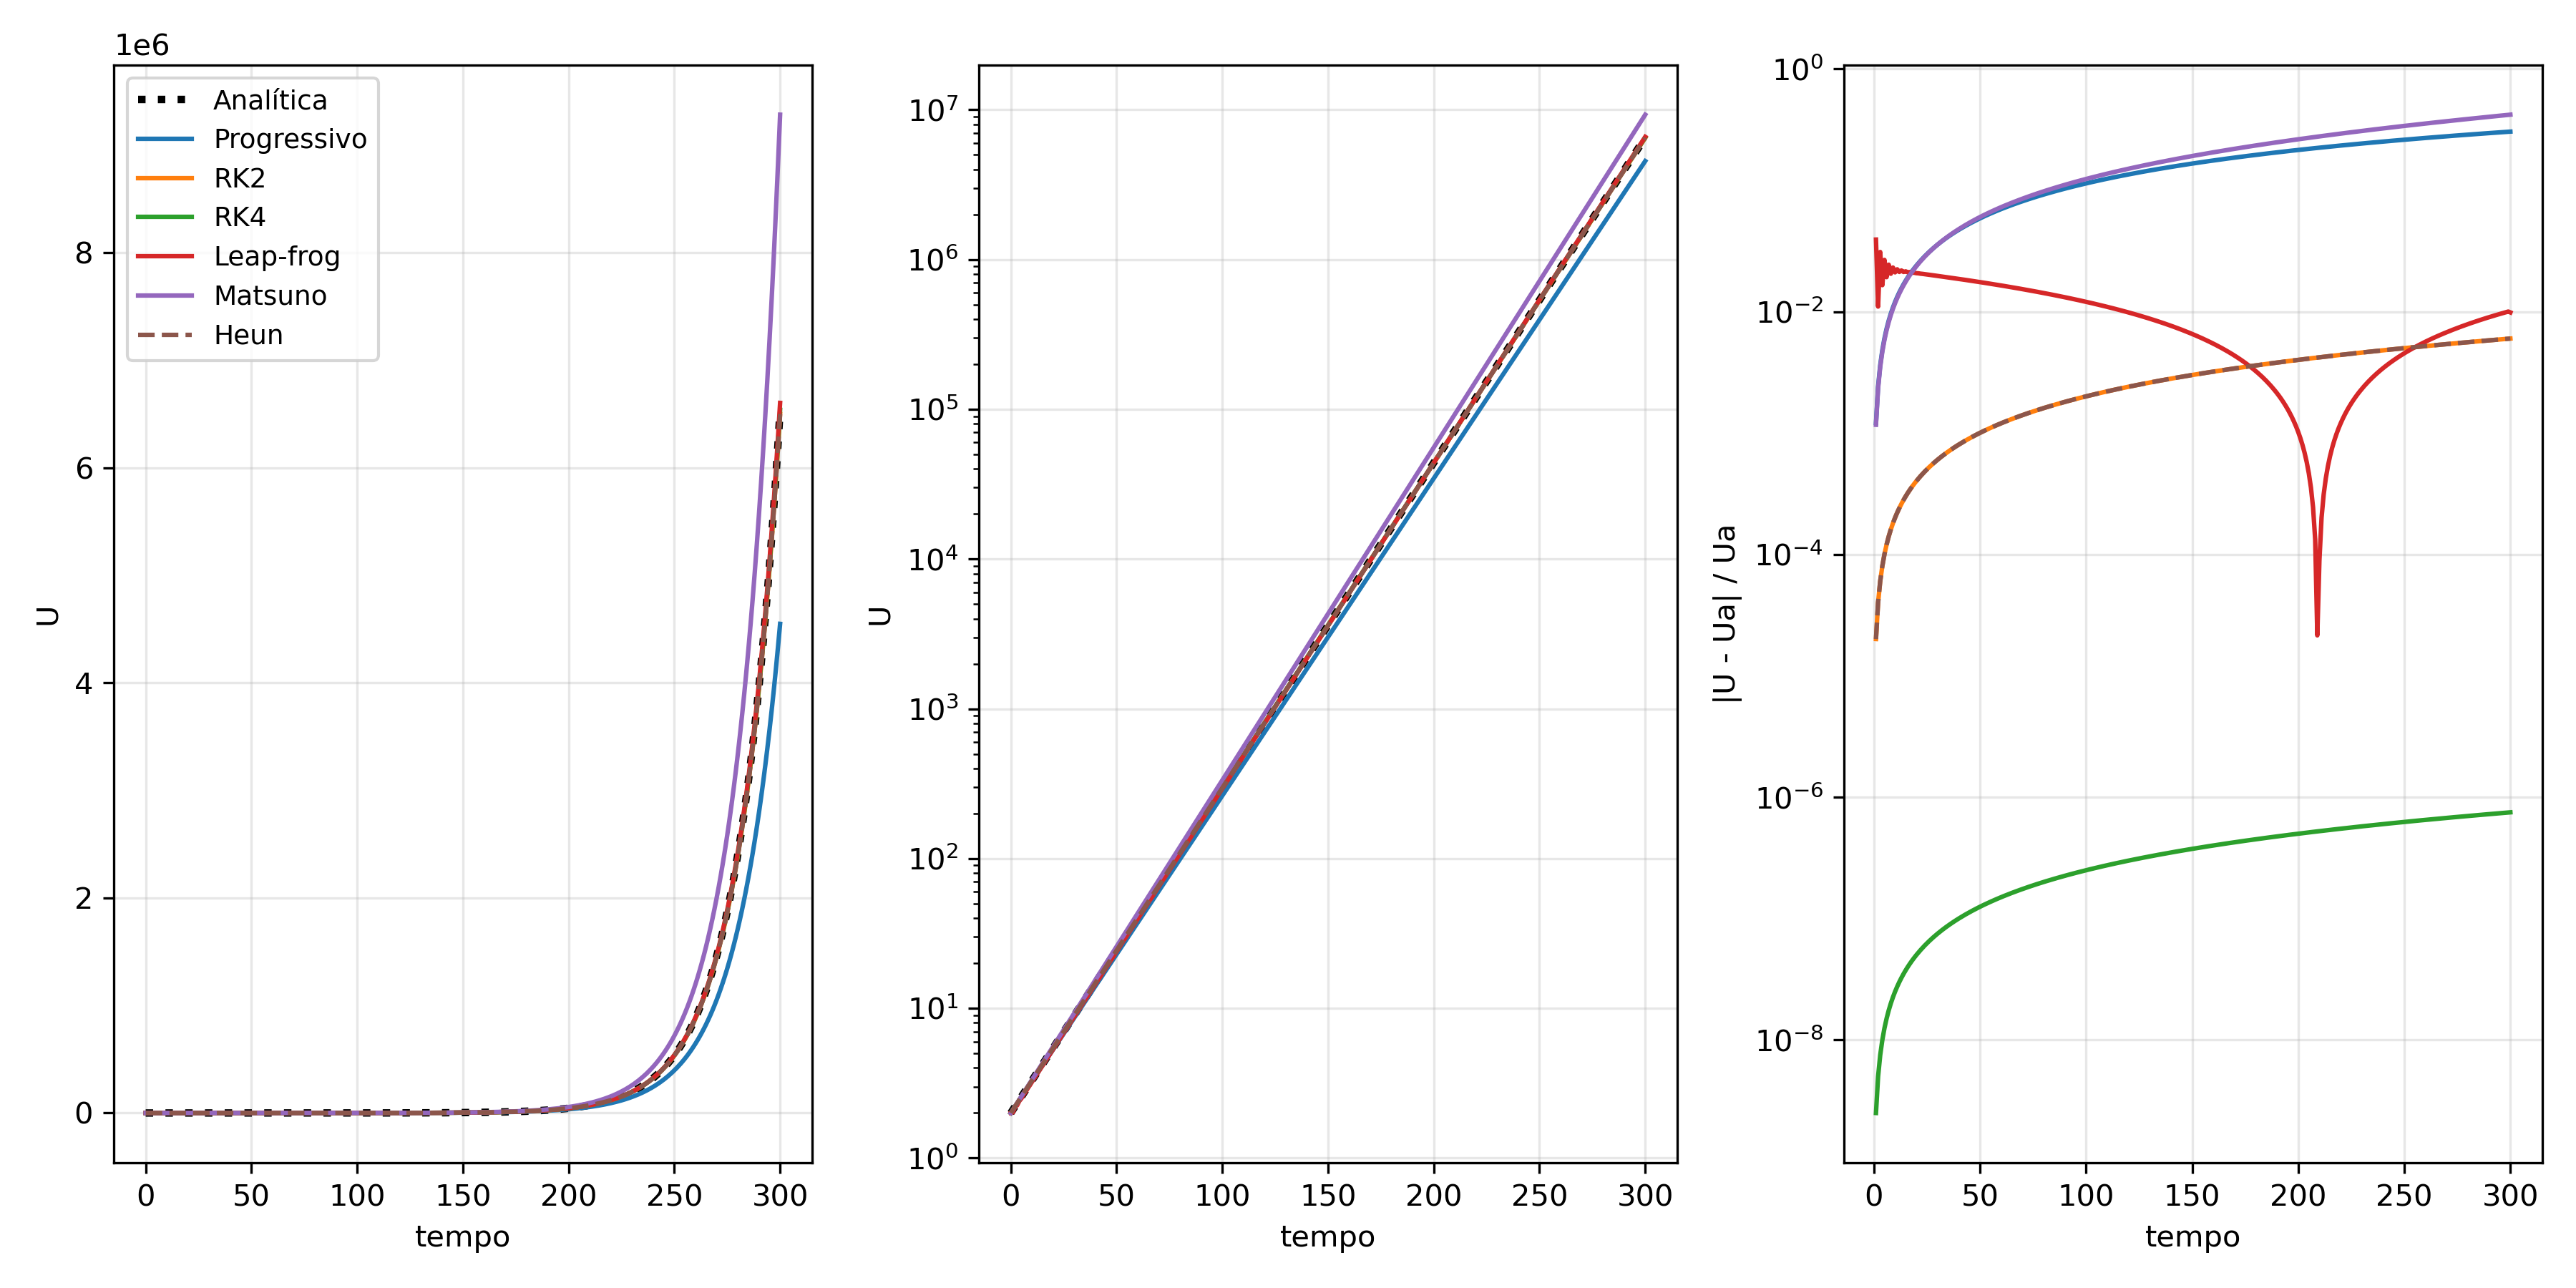
\includegraphics[width=\textwidth]{../resultado_dt1.png}
  \caption{Solução da Equação~\ref{eq:cresc} para $\Delta t = 1$, analítica e pelos esquemas progressivo, Runge-Kutta de 2ª ordem (RK2), Runge-Kutta de 4ª ordem (RK4), leap-frog, Matsuno e Heun. O painel da esquerda apresenta os resultados em escala linear e o do meio em escala logarítmica. O painel da direita apresenta o erro relativo das aproximações estudadas.}
  \label{fig:dt1}
\end{figure}

\begin{figure}[H]
  \centering
  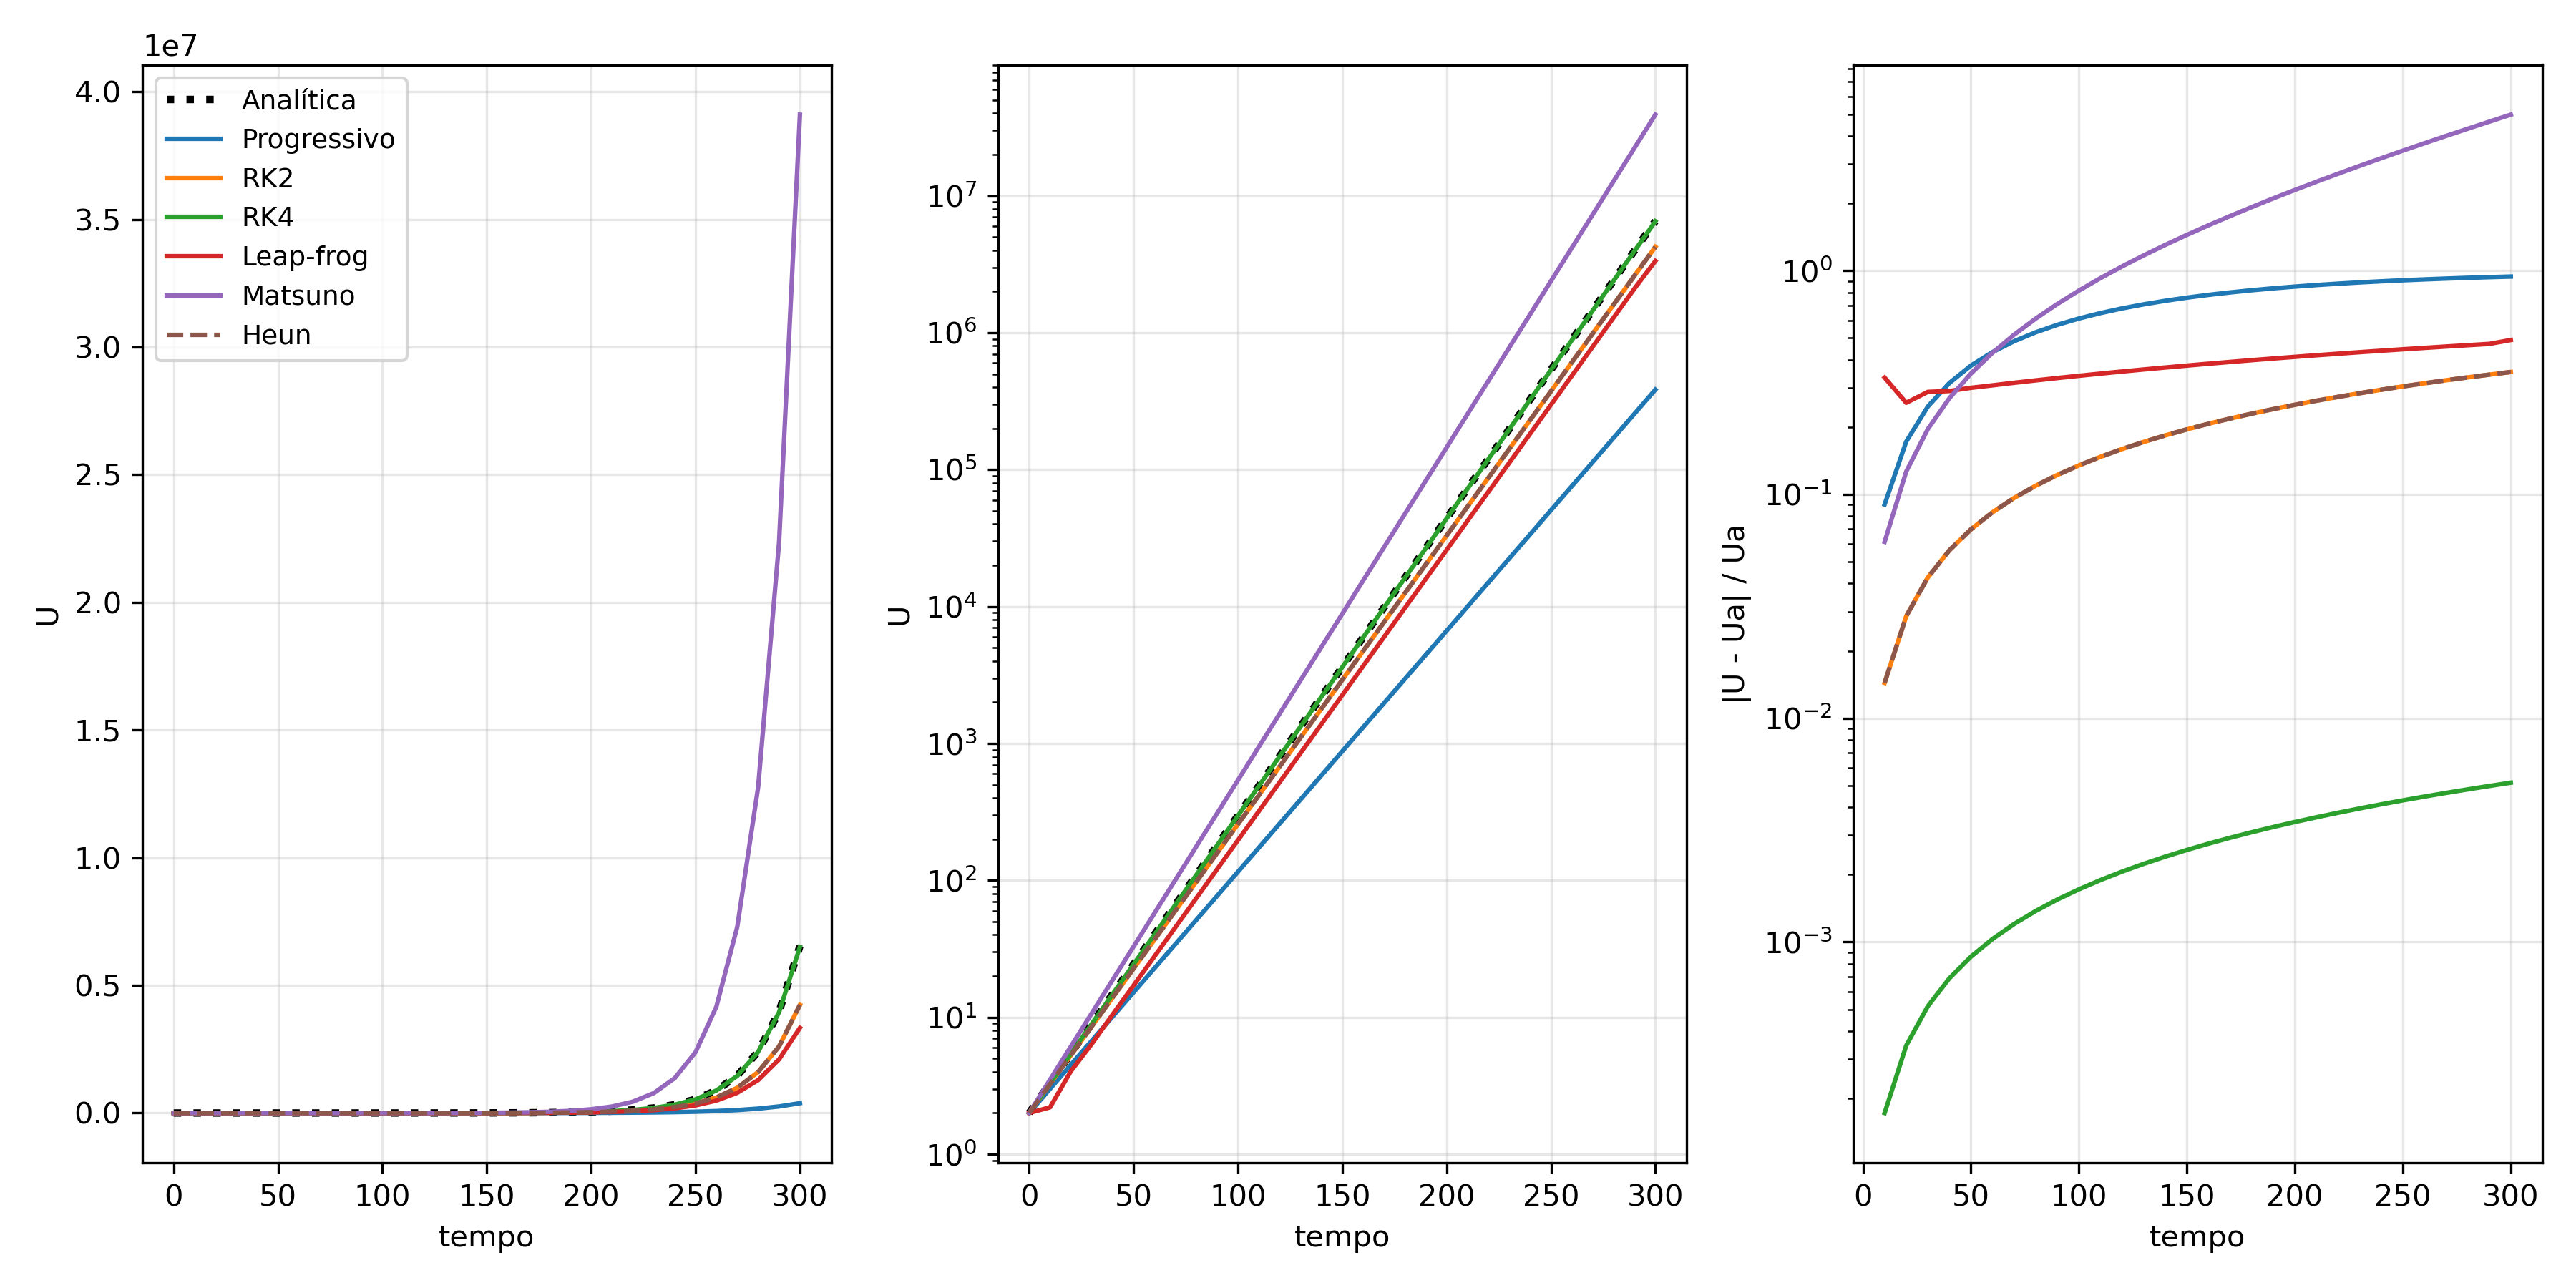
\includegraphics[width=\textwidth]{../resultado_dt10.png}
  \caption{Como na Figura~\ref{fig:dt1}, mas para $\Delta t = 10$.}
  \label{fig:dt10}
\end{figure}

\begin{table}[htbp]
\centering
\caption{Erro relativo de cada esquema para $\Delta t = 1$ e $\Delta t = 10$.}
\label{tab:erros}
\begin{tabular}{lcccc}
\hline
 & \multicolumn{2}{c}{$\Delta t = 1$} & \multicolumn{2}{c}{$\Delta t = 10$} \\
Esquema & $t = 300$ & Médio & $t = 300$ & Médio \\
\hline
Progressivo & $3{,}0\times10^{-1}$ & $1{,}6\times10^{-1}$ & $9{,}4\times10^{-1}$ & $6{,}8\times10^{-1}$ \\
RK2         & $6{,}0\times10^{-3}$ & $3{,}0\times10^{-3}$ & $3{,}5\times10^{-1}$ & $1{,}9\times10^{-1}$ \\
RK4         & $7{,}5\times10^{-7}$ & $3{,}8\times10^{-7}$ & $5{,}2\times10^{-3}$ & $2{,}7\times10^{-3}$ \\
Leap-frog   & $9{,}9\times10^{-3}$ & $9{,}6\times10^{-3}$ & $4{,}9\times10^{-1}$ & $3{,}8\times10^{-1}$ \\
Matsuno     & $4{,}2\times10^{-1}$ & $2{,}0\times10^{-1}$ & $5{,}0$             & $1{,}9$ \\
Heun        & $6{,}0\times10^{-3}$ & $3{,}0\times10^{-3}$ & $3{,}5\times10^{-1}$ & $1{,}9\times10^{-1}$ \\
\hline
\end{tabular}
\end{table}

Em geral, o erro relativo cresce ao longo da integração, pois o erro do fator de amplificação se acumula a cada passo de tempo. A exceção é o leap-frog com $\Delta t = 1$, discutido adiante. O erro também aumenta fortemente com $\Delta t$. Ao reduzir o passo de tempo de 10 para 1, o erro final diminuiu cerca de 60 vezes para o RK2 e cerca de 7000 vezes para o RK4. Para o Matsuno, de 1ª ordem, a redução foi de cerca de 12 vezes. Para o progressivo, a redução foi de apenas 3 vezes: com $\Delta t = 10$ ($g\Delta t = 0{,}5$), seu erro relativo já se aproxima do limite de 100\%.

O esquema de Runge-Kutta de 4ª ordem apresentou os melhores resultados para os dois passos de tempo. Com $\Delta t = 10$, seu erro foi comparável ou ligeiramente inferior ao dos demais esquemas com $\Delta t = 1$, ou seja, o RK4 atinge a mesma precisão com um passo de tempo dez vezes maior.

Os esquemas RK2 e Heun produziram resultados idênticos. Para uma equação linear, ambos possuem o mesmo fator de amplificação, $1 + g\Delta t + (g\Delta t)^2/2$. Por serem de 2ª ordem, apresentaram bom desempenho com $\Delta t = 1$, mas se degradaram consideravelmente com $\Delta t = 10$.

O leap-frog apresentou um comportamento distinto dos demais. Por causa do passo inicial, que repete a condição inicial, a solução parte atrasada em relação à analítica. Nos primeiros passos, a solução alterna entre valores acima e abaixo da tendência, gerando as oscilações no erro no início do painel direito da Figura~\ref{fig:dt1}. Essas oscilações correspondem ao modo computacional do esquema, que é rapidamente amortecido pelo filtro de Asselin. Um comportamento interessante deste esquema é o mínimo absoluto do erro próximo ao passo de tempo 200 no caso $\Delta t = 1$, que pode ser explicado à luz deste filtro, que faz com que a solução numérica cresça mais rápido que a analítica, alcançando-a próximo ao passo 200, e então passe a superestimá-la. Como se analisa o erro relativo, que leva em consideração o módulo da diferença, essa troca de sinal aparece no gráfico como um mínimo pontual, e não como um ganho real de precisão.

O esquema progressivo subestima o crescimento, pois $1 + g\Delta t < e^{g\Delta t}$. O esquema de Matsuno, ao contrário, superestima o crescimento, pois seu fator de amplificação, $1 + g\Delta t + (g\Delta t)^2$, é maior que o exato. Por isso foi o pior esquema neste problema, chegando a um erro de aproximadamente 500\% ao final da integração com $\Delta t = 10$. 

% ---------- Conclusão ----------
\section{Conclusão}

O esquema de Runge-Kutta de 4ª ordem foi o mais preciso para os dois passos de tempo. Os esquemas RK2/Heun e leap-frog tiveram desempenho intermediário, e os esquemas de 1ª ordem (progressivo e Matsuno) tiveram os maiores erros, especialmente para $\Delta t = 10$.

% ---------- Nota sobre IA ----------
\vspace{1.2em}
\noindent\fbox{\parbox{\dimexpr\textwidth-2\fboxsep-2\fboxrule}{\small\setstretch{1.1}%
\textbf{Uso de IA:} a ferramenta Claude (Anthropic) foi utilizada na revisão do texto e do código, e na formatação em \LaTeX.}}

\end{document}